\documentclass[aspectratio=169]{beamer}
\usetheme{simple}

\input{preamble/preamble.tex}
\input{preamble/preamble_math.tex}
% \input{preamble/preamble_acronyms.tex}

\title{Recurrent Neural Networks}
\subtitle{STATS305B: Applied  Statistics II}
\author{Scott Linderman}
\date{\today}


\begin{document}


\maketitle

\begin{frame}{Last Time...}
    \begin{itemize}
        \item Transformers
        \item Attention
        \item Some tricks
    \end{itemize}
\end{frame}

\begin{frame}{Today...}
    \textbf{Outline:}
    \begin{itemize}
        \item Recurrent Neural Networks
        \item Backpropagation Through Time
        \item Vanishing Gradients and Gated RNNs
        \item Other Variations and Uses of RNNs
        \item Revisiting HMMs
        \item Linear RNNs and Parallel Inference
    \end{itemize}
    \vspace{1em}
\end{frame}



\begin{frame}[t,allowframebreaks]{Autoregressive Models}\label{autoregressive-models}

Consider a sequence of observations
\(\mbx_{1:T} = (\mbx_1, \ldots, \mbx_T)\) with each
\(\mbx_t \in \reals^D\). We can always factor a joint distribution over
observation into a product of conditionals using the chain rule,
\begin{align*}
p(\mbx_{1:T}) &= p(\mbx_1) \prod_{t=2}^T p(\mbx_t \mid \mbx_{1:t-1}).
\end{align*} This is called an \textbf{autoregressive model} since the
conditional of \(\mbx_t\) depends only on previous observations
\(\mbx_{1}, \ldots, \mbx_{t-1}\).

Autoregressive models are well-suited to sequential modeling since they
make forward generation or \emph{forecasting} easy. As long as we have
access to the conditionals, we can sample forward indefinitely.

The question is, how should we parameterize these conditional
distributions? It looks challenging since each one takes in a
variable-length history of previous observations.

\end{frame}

\begin{frame}[t,allowframebreaks]{Recurrent Neural
Networks}\label{recurrent-neural-networks-1}

Recurrent Neural Networks (RNNs) are autoregressive models in which the
conditional distributions are functions of a finite-dimensional
\textbf{hidden state}, \(\mbh_t \in \reals^K\), \begin{align*}
p(\mbx_t \mid \mbx_{1:t-1}) &= p(\mbx_t \mid g(\mbh_t; \mbtheta)).
\end{align*} The hidden state is updated with each new observation as,
\begin{align*}
\mbh_{t+1} &= f(\mbh_t, \mbx_t; \mbtheta).
\end{align*}

\textbf{Defining Property of an RNN} 
\emph{The conditional distribution over the next observation is a function of hidden state. The hidden state is updated recursively, and its size is fixed regardless of the sequence length.} 

\end{frame}

\begin{frame}[t,allowframebreaks]{Vanilla RNNs}\label{vanilla-rnns}

The standard, ``vanilla'' RNN consists of a linear-nonlinear state
update. For example, \begin{align*}
f(\mbh_t, \mbx_t; \mbtheta)
&= \tanh \left(\mbW \mbh_t + \mbB \mbx_t \right),
\end{align*} where - \(\mbW \in \reals^{K \times K}\) are the dynamics
weights, - \(\mbB \in \reals^{K \times D}\) are the input weights, -
\(\tanh(\cdot)\) is the hyperbolic tangent function.

\textbf{Hyperbolic Tangent and the Logistic Function}
The hyperbolic tangent function equivalent is typically written
as, 
\begin{align*}
\tanh(a) &= \frac{e^a - e^{-a}}{e^a + e^{-a}}. 
\end{align*} 
We can rewrite $\tanh$ as, 
\begin{align*}
\tanh(a) &= 1 - \frac{2e^{-a}}{e^a + e^{-a}} \\
% &= 1 - \frac{2}{e^{2a} + 1} \\
&= 1 - 2 \sigma(-2a) \\
&= 1 - 2 (1 - \sigma(2a)) \\
&= 2 \sigma(2a) - 1.
\end{align*} 
Thus, we see that the the hyperbolic tangent is simply a
scaled and shifted logistic function. 

The ``read-out'' of a vanilla RNN is typically a simple linear or
generalized linear model, depending on the type of observations. For
example, \begin{align*}
g(\mbh_t, \mbx_t; \mbtheta) &= \mbC \mbh_t + \mbd,
\end{align*} where \(\mbC \in \reals^{D \times K}\) is the read-out
weight matrix and \(\mbd \in \reals^D\) is the bias.

Let \(\mbtheta = (\mbW, \mbB, \mbC, \mbd)\) denote the set of
parameters.
\end{frame}

\begin{frame}[t,allowframebreaks]{Theoretical Neuroscience}\label{theoretical-neuroscience}

In machine learning, RNNs are useful function
approximators for sequential data. In neuroscience, they
have a long history as theoretical models of biological computation.

The hidden state \(\mbh_t \in \reals^K\) corresponds to
the relative \textbf{firing rates} of \(K\) neurons. With a $\tanh$ nonlinearity, \(\mbh_t \in (-1, 1)^K\), and negative rates don't
make sense. Instead, we think of \(\mbh_t\) as an offset to a
baseline firing rate.

The dynamics weights correspond to \textbf{synaptic connections}, with
positive weights as excitatory synapses and negative weights as
inhibitory. When a presynaptic neuron spikes, it induces an electrical
current in postsynaptic neurons. The
activation \(\mbW \mbh_t\) is the \textbf{input current}
from other neurons.

As a neuron receives input current, its voltage steadily increases until
it reaches a \textbf{threshold}, at which point the voltage spikes and
the neuron fires an \textbf{action potential}. These spikes induce
currents on downstream neurons, as described above. 

After a cell fires,
there is a short \textbf{refractory period} before the neuron can spike
again. Thus, there is an upper bound on firing rates, which the
hyperbolic tangent is meant to capture.

\end{frame}

\begin{frame}[t,allowframebreaks]{Backpropagation Through
Time}\label{backpropagation-through-time}

Artificial RNNs are trained using stochastic gradient descent (SGD) to
minimize the negative log likelihood, 
\begin{align*}
\cL(\mbtheta)
&= - \sum_{t=1}^T \log p(\mbx_t \mid \mbx_{1:t-1}) \\
&= - \sum_{t=1}^T \log p(\mbx_t \mid g(\mbh_t; \mbtheta)) \\
&= - \sum_{t=1}^T \log p(\mbx_t \mid g(f(\mbh_{t-1}, \mbx_{t-1}; \mbtheta); \mbtheta)) \\
&= - \sum_{t=1}^T \log p(\mbx_t \mid g(f(\cdots f(\mbh_{1}, \mbx_{1}; \mbtheta) \cdots, \mbx_{t-1}; \mbtheta); \mbtheta)).
\end{align*} 
Now, you would simply use automatic differentiation to
compute the necessary gradients to minimize this loss, but we can gain
some insight by working them out manually. 

With some algebra, we can
show that the Jacobian of the loss with respect to the dynamics weights
(other parameters are similar) is, 
\begin{align*}
\frac{\partial \cL(\mbtheta)}{\partial \mbW} &= \sum_{t=1}^T \frac{\partial \cL(\mbtheta)}{\partial \mbh_t} \frac{ \partial \mbh_t}{\partial \mbW}
\end{align*} 
We need the Jacobian of the loss with respect to the hidden
states. These can be computed recursively by \textbf{backpropagation
through time (BPTT)}, 
\begin{align*}
\frac{\partial \cL(\mbtheta)}{\partial \mbh_t} 
&= \frac{\partial \cL(\mbtheta)}{\partial \mbh_{t+1}} \frac{\partial \mbh_{t+1}}{\partial \mbh_t} - \frac{\partial \log p(\mbx_t \mid g(\mbh_t; \mbtheta))}{\partial \mbh_t}
\end{align*} 
For a vanilla RNN, the Jacobian of the next state with
respect to the current state is, \begin{align*}
\frac{\partial \mbh_{t+1}}{\partial \mbh_t} 
&= \diag \left(1 - \mbh_{t+1}^2 \right) \mbW
\end{align*} since \(\frac{\dif}{\dif a}\tanh(a) = 1 - \tanh(a)^2\).

\end{frame}

\begin{frame}[t,allowframebreaks]{BPTT is a linear dynamical system} 
    
The ``state'' of the BPTT recursions is the Jacobian, or equivalently its transpose, the
gradient
\(\mbs_t \triangleq \left(\frac{\partial \cL(\mbtheta)}{\partial \mbh_t}\right)^\top\).
This state obeys a linear dynamical system, \begin{align*}
\mbs_t &= \mbA_t \mbs_{t+1} + \mbb_t
\end{align*} where
\(\mbA_t = \left(\frac{\partial \mbh_{t+1}}{\partial \mbh_t} \right)^\top\)
and
\(\mbb_t = - \left(\frac{\partial \log p(\mbx_t \mid g(\mbh_t; \mbtheta))}{\partial \mbh_t} \right)^\top\).
\end{frame}

\begin{frame}[t,allowframebreaks]{Biological Plausibility}
    
Backpropagation is the most effective way we know of to train artificial
RNNs, so it's reasonable to think that the brain might be using a
similar learning algorithm. 

Unfortunately, it's not clear how the
backpropagation through time algorithm could be implemented by a neural
circuit. 

The multiplication by \(\mbA_t\) in the gradient recursions
amounts to passing information backward across synapses, and canonical
synaptic models don't have mechanisms to do this. 

Recent years have seen
a substantial amount of research into biologically plausible mechanisms
of backpropagation. 
\end{frame}

\begin{frame}[t,allowframebreaks]{Vanishing Gradients}\label{vanishing-gradients}

When the Jacobians \(\mbA_t\) have small eigenvalues (\(\ll 1\)), we run
into problems of \textbf{vanishing gradients}. 

Consider the case of a
linear RNN in which the \(\tanh\) is replaced with identity: then the
Jacobians are \(\mbA_t = \mbW^\top\) for all time steps. 

If the
eigenvalues of \(\mbW\) are much less than one, the gradients will decay
to zero exponentially quickly, absent strong inputs \(\mbb_t\).

Vanishing gradients are especially problematic when \(\mbx_t\) depends
on much earlier observations, \(\mbx_s\) for \(s \ll t\). In that case,
the hidden state must propagate information about \(\mbx_s\) for many
time steps during the forward pass, and likewise, the gradient must pass
information backward many timesteps during the backward pass. 

If the
weights have small eigenvalues, those gradients will decay and the
learning signal will fail to propagate.
\end{frame}

\begin{frame}[t,allowframebreaks]{Gated RNNs}\label{gated-rnns}

One way to combat the vanishing gradient problem is by modifying the RNN
architecture. Architectures like \textbf{long short-term memory (LSTM)}
networks achieve this via gated units.

\begin{figure}
\centering
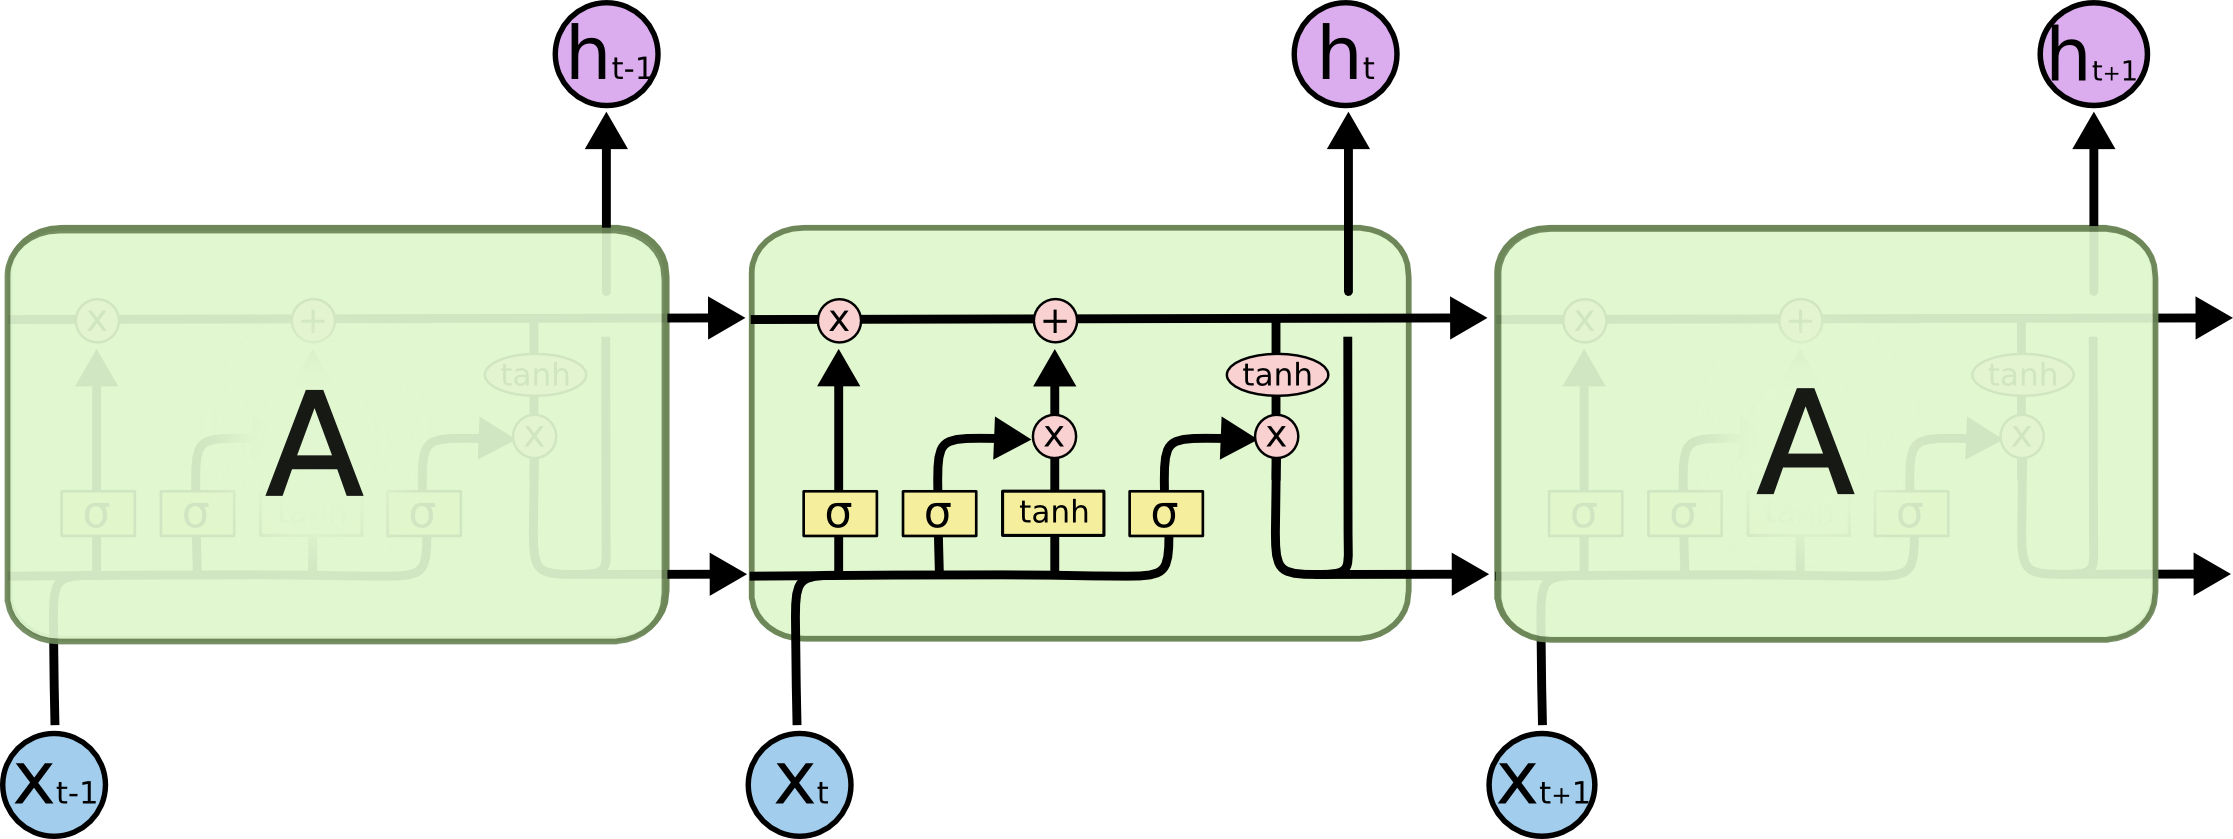
\includegraphics[width=0.75\textwidth]{15_rnns/lstm.png}
\caption{An LSTM cell. Figure from \url{https://colah.github.io/posts/2015-08-Understanding-LSTMs/}.}
\end{figure}

An LSTM has internal (aka ``cell'') states \(\mbc_t \in \reals^K\) and
hidden states \(\mbh_t \in \reals^K\). The internal states follow
\textbf{conditionally linear} dynamics, 
\begin{align*}
\mbc_{t} &= \mbF_t \mbc_{t-1} + \mbb_t
\end{align*} 
where 
\begin{align*}
\mbF_t &= \diag(f_{t,1}, \ldots, f_{t,K}) \\
f_{t,k} &= \sigma(\mbW^{(f)} \mbh_{t-1} + \mbB^{(f)} \mbx_{t-1}).
\end{align*} 
The bounded entries \(f_{t,k} \in [0,1]\) ensure stability.
When \(f_{t,k} \approx 1\), the state is propagated, and when
\(f_{t,k} \approx 0\), the state is forgotten. 

Thus,
\(\mb{f}_t = (f_{t,1}, \ldots, f_{t,K})^\top \in [0,1]^K\) are called the
\textbf{forget gates}, and they are parameterized by the matrices
\(\mbW^{(f)}\) and \(\mbB^{(f)}\).

The affine term is determined by, 
\begin{align*}
\mbb_t &= \mbg_t \odot \mbi_t \\
\mbg_t &= \sigma(\mbW^{(g)} \mbh_{t-1} + \mbB^{(g)} \mbx_{t-1}) \\
\mbi_t &= \sigma(\mbW^{(i)} \mbh_{t-1} + \mbB^{(i)} \mbx_{t-1})
\end{align*} 
The vector \(\mbg_t \in [0,1]^K\) plays the role of an
\textbf{input gate}, and the input s themselves are given by
\(\mbi_t \in [0,1]^K\).

Finally, the hidden states \(\mbh_t\) are gated functions of the
internal state passed through a nonlinearity, 
\begin{align*}
\mbh_t &= \mbo_t \odot \tanh(\mbc_t) \\
\mbo_t &= \sigma(\mbW^{(o)} \mbh_{t-1} + \mbB^{(o)} \mbx_{t-1})
\end{align*} 
where \(\mbo_t \in [0,1]^K\) are the \textbf{output gates}.
As in a vanilla RNN, the final prediction depends on a (generalized)
linear function of the hidden state, \(g(\mbh_t; \mbtheta)\).

We can think of an LSTM as an RNN that operates on an extended state
\((\mbc_t, \mbh_t) \in \reals_+^K \times [-1, 1]^K\). The forget gates
let the eigenvalues of \(\mbF_t\) to be close to one, allowing cell
states to be propagated for long periods of time on the forward pass,
and gradients to be backpropagated without vanishing on the backward
pass.

There are many variants of gated RNNs. Besides the LSTM, the most
commonly used in the gated recurrent unit (GRU), which has a slightly
simplified architecture. See Goodfellow et al. (2016), Ch. 10,for more detail.
\end{frame}

\begin{frame}[t,allowframebreaks]{Other Variations and Uses of
RNNs}\label{other-variations-and-uses-of-rnns}

We motivated RNNs from an autoregressive modeling persepective, but they
are useful in other sequential data settings as well. 

For example,
suppose we want to predict the sentiment of a review \(y \in \reals\)
given a variable-length sequence of input words \(\mbx_{1:T}\). 

We can
use an RNN to summarize the input sequence in terms of a hidden state
for prediction, 
\begin{align*}
p(y \mid \mbx_{1:T}) &= p(y \mid g(\mbh_T; \mbtheta)).
\end{align*}
\end{frame}

\begin{frame}[t,allowframebreaks]{Sequence to Sequence
Models}\label{sequence-to-sequence-models}

Sometimes we want to map one sequence \(\mbx_{1:T}\) to another sequence
\(\mby_{1:T'}\). The sequences may be of different length; e.g., when we
want to translate a sentence from English to French. 

Again, we can train
an \textbf{encoder} RNN to produce a hidden state \(\mbh_T\) that then
becomes the initial condition for a \textbf{decoder} RNN that generates
the output sequence. 

Formally, 
\begin{align*} 
p(\mby_{1:T'} \mid \mbx_{1:T}) 
&= \prod_{t=1}^{T'} p(\mby_{t} \mid \mby_{1:t-1}, \mbx_{1:T}) \\
&= \prod_{t=1}^{T'} p(\mby_{t} \mid \mbh'_t, \mbh_T)
\end{align*} 
where \(\mbh_T\) is the output of an RNN that processed
\(\mbx_{1:T}\), and \(\mbh'_t\) is the state of an RNN that runs over
\(\mby_{1:T}\).
\end{frame}

\begin{frame}[t,allowframebreaks]{Bidirectional RNNs}\label{bidirectional-rnns}

In the example above, one challenge is that the hidden state \(\mbh_T\)
obtained by processing \(\mbx_{1:T}\) may not adequately represent early
inputs like \(x_1\). 

For these purposes, you can use a
\textbf{bidirectional RNN} that runs one recursion forward
\(\mbx_1, \ldots, \mbx_T\) and another backward
\(\mbx_T, \ldots, \mbx_1\) to produce two hidden states at each time
\(t\). 

These combined states can then be passed into the decoder.
\end{frame}

\begin{frame}[t,allowframebreaks]{Deep RNNs}\label{deep-rnns}

As with deep neural networks that stack layer upon layer, we can stack
RNN upon RNN to construct a deeper model. 

In such models, the outputs of
one layer, \(g(\mbh_t^{(i)}; \mbtheta^{(i)})\) become the inputs to the
next layer, \(\mbx_t^{(i+1)}\). 

Then we can backpropagate gradients
through the entire stack to train the model.
\end{frame}

\begin{frame}[t,allowframebreaks]{HMMs Are RNNs Too!}\label{hmms-are-rnns-too}

We presented
Hidden Markov Models (HMMs) as latent variable models with hidden states
\(\mbz_{1:T}\) and observations \(\mbx_{1:T}\),
but we can also view them as an autoregressive model,
\begin{align*}
p(\mbx_t \mid \mbx_{1:t-1}) 
&= \sum_{k=1}^K p(z_t=k \mid \mbx_{1:t-1}) \, p(\mbx_t \mid z_t=k) \\
&= \sum_{z_t} \overline{\alpha}_{t,k} \, p(\mbx_t \mid z_t=k)
\end{align*} 
where, \(\overline{\mbalpha}_t \in \Delta_{K-1}\) are the
\textbf{normalized forward messages} from the forward-backward
algorithm. 

They followed a simple recursion, 
\begin{align*}
\overline{\mbalpha}_{t+1} &= \mbP^\top \left( \frac{\overline{\mbalpha}_t \odot \mbl_t}{\overline{\mbalpha}_t^\top \mbl_t} \right)
\end{align*} 
with \(\mbl_t \in \reals^K\) is the vector of likelihoods
with entries \(l_{t,k} = p(\mbx_t \mid z_t=k)\) and
\(\mbP \in \reals^{K \times K}\) is the transition matrix.
\end{frame}

\begin{frame}[t,allowframebreaks]{Categorical HMMs}\label{categorical-hmms}

Consider an HMM with categorical emissions, 
\begin{align*}
p(\mbx_t \mid z_t) &= \mathrm{Cat}(\mbx_t \mid \mbc_{z_t}),
\end{align*} 
where \(\mbx_t\) is a one-hot encoding of a variable that
takes values in \(\{1,\ldots,V\}\), and \(\mbc_k \in \Delta_{V-1}\) for
\(k=1,\ldots,K\) are pmfs. 

Define the matrix of likelihoods
\(\mbC \in \reals^{V \times K}\) to have columns \(\mbc_k\),
\begin{align*}
\mbC &=
\begin{bmatrix}
| & & | \\
\mbc_1 & \cdots & \mbc_K \\
| & & | 
\end{bmatrix}.
\end{align*} 
The HMM parameters are \(\mbtheta = (\mbP, \mbC)\). (Assume
the initial distribution is fixed, for simplicity.)

For a categorical HMM, we can write the likelihoods as
\(\mbl_t = \mbC^\top \mbx_t\) so that the the forward recursions
simplify to, 
\begin{align*}
\overline{\mbalpha}_{t+1} 
&= \mbP^\top \left( \frac{\overline{\mbalpha}_t \odot \mbC^\top \mbx_t}{\overline{\mbalpha}_t^\top \mbC^\top \mbx_t} \right) \\
&= f(\overline{\mbalpha}_t, \mbx_t; \mbtheta)
\end{align*}
 Likewise, the autoregressive distributions reduce to,
\begin{align*}
p(\mbx_t \mid \mbx_{1:t-1}) 
&= \mathrm{Cat}(\mbx_t \mid \mbC \overline{\mbalpha}_t) \\
&= \mathrm{Cat}(\mbx_t \mid g(\overline{\mbalpha}_t; \mbtheta)).
\end{align*} 
Framed this way, a categorical HMM can be seen as a simple
recurrent neural network!
\end{frame}

\begin{frame}[t,allowframebreaks]{A Cool Trick for Computing the
Gradients}\label{a-cool-trick-for-computing-the-gradients}

This formulation suggests that we could estimate the parameters of an
HMM by directly maximizing the log likelihood, 
\begin{align*}
\cL(\mbtheta) &= \log p(\mbx_{1:T}; \mbtheta) = \sum_{t=1}^T \log p(\mbx_t \mid \mbx_{1:t-1}; \mbtheta).
\end{align*} 
With automatic differentiation at our disposal, this sounds
like it might be a lot easier!

Let's pursue this idea a little further. First, we'd prefer to do
unconstrained optimization, so let's parameterize the model in terms of
\(\log \mbP\) and \(\log \mbC\). 
\end{frame}

\begin{frame}[t,allowframebreaks]{Aside: The softmax function}
When we need the constrained versions,
we will just apply the softmax to obtain simplex vectors: 
\begin{align*}
\mathrm{softmax}(\log \mbc_k) 
&= \left(
    \frac{e^{\log c_{k,1}}}{\sum_{v=1}^V e^{\log c_{k,v}}}, 
    \ldots,
    \frac{e^{\log c_{k,V}}}{\sum_{v=1}^V e^{\log c_{k,v}}}
 \right)^\top
\end{align*}

Softmax is translation invariant Note that the softmax
operation is translation invariant, 
\begin{align*}
\mathrm{softmax}(\log \mbc_k) &=
\mathrm{softmax}(\log \mbc_k + a) 
\end{align*} for any constant \(a \in \reals\). 

Thus, we will call our
optimization variables \(\log \mbC\) and \(\log \mbP\), but they are not
actually the log of matrices with simplex columns or rows; they are
unconstrained parameters that become properly normalized via the
softmax. 
\end{frame}

\begin{frame}[t,allowframebreaks]{A Cool Trick for Computing the
    Gradients}\label{a-cool-trick-for-computing-the-gradients}
To maximize the likelihood with gradient ascent, we need the Jacobians,
\(\frac{\partial \cL(\mbtheta)}{\partial \log \mbP}\) and
\(\frac{\partial \cL(\mbtheta)}{\partial \log \mbC}\). For the RNNs
above, we computed them using backpropagation through time, but here we
can use an even cooler trick.

First, note that the posterior distribution in an HMM can be written as
an exponential family, 
\begin{align*}
p(\mbz_{1:T} \mid \mbx_{1:T}; \mbtheta) 
&= \exp \left\{ \log p(\mbz_{1:T}, \mbx_{1:T}; \mbtheta) - \log p(\mbx_{1:T}; \mbtheta) \right\} \\
&= \exp \left\{ 
    \log p(z_1; \mbpi_0) 
    + \sum_{t=2}^T \log p(z_t \mid z_{t-1}; \mbP) 
    + \sum_{t=1}^T \log p(\mbx_t \mid z_{t}; \mbC) 
    - \log p(\mbx_{1:T}; \mbtheta)
    \right\} \\
&= \exp \bigg\{ 
    \sum_{k=1}^K \langle \bbI[z_1 =k], \log \pi_{0,k} \rangle \\
    &\hspace{6em}
    + \sum_{t=2}^T \sum_{i=1}^K \sum_{j=1}^K \langle \bbI[z_{t-1}=i \wedge z_{t} = j],  \log P_{i,j} \rangle \\
    &\hspace{12em}
    + \sum_{t=1}^T \sum_{v=1}^V \sum_{k=1}^K \langle \bbI[x_t = v \wedge z_t = k], \log C_{v,k} \rangle \\
    &\hspace{18em} - A(\mbtheta)
    \bigg\} 
\end{align*} 
where the log marginal likelihood
\(A(\mbtheta) = \log p(\mbx_{1:T}; \mbtheta)\) is the log normalizer.
\end{frame}

\begin{frame}[t,allowframebreaks]{A Cool Trick for Computing the
    Gradients}\label{a-cool-trick-for-computing-the-gradients}
Recall that for exponential family distributions, gradients of the log
normalizer yield expected sufficient statistics. Thus, 
\begin{align*}
\frac{\partial A(\mbtheta)}{\partial \log C_{v,k}} 
&= \sum_{t=1}^T \bbI[x_{t} = v] \cdot \bbE_{p(\mbz_{1:T} \mid \mbx_{1:T}; \mbtheta)} \left[\bbI[z_{t}=k] \right]
\end{align*} 
and 
\begin{align*}
\frac{\partial A(\mbtheta)}{\partial \log P_{i,j}} 
&= \sum_{t=2}^T \bbE_{p(\mbz_{1:T} \mid \mbx_{1:T}; \mbtheta)} \left[ \bbI[z_{t-1}=i \wedge z_{t} = j] \right]
\end{align*} 
The gradients are essentially the posterior marginals and
pairwise marginals we computed in the EM algorithm!

In the M-step of EM, we solve for the parameters that satisfy the
constrained optimality conditions, whereas in SGD we just take a step in
the direction of the gradient. EM tends to converge must faster in
practice for this reason.
\end{frame}

\begin{frame}[t,allowframebreaks]{Linear RNNs}\label{linear-rnns}

Consider the special case of \emph{linear} RNNs,
\begin{align*}
\mbh_t &= \mbA \mbh_{t-1} + \mbB \mbx_t.
\end{align*}
with outputs \(\mby_t = \mbC \mbh_t + \mbd\).

Since a linear operators compose, the mapping from $\mbx_{1:T}$ to $\mby_{1:T}$ is a linear function,
\begin{align*}
\mby_t 
&= \mbC \mbh_t + \mbd \\
&= \mbC (\mbA \mbh_{t-1} + \mbB \mbx_t) + \mbd \\
&= \mbC (\mbA (\mbA \mbh_{t-2} + \mbB x_{t-1}) + \mbB \mbx_t) + \mbd \\
% &\vdots \\
&= \mbC \left(\sum_{s=0}^{t-1} \mbA^s \mbB \mbx_{t-s} \right) + \mbd 
\end{align*} with the convention that \(\mbh_0 = 0\).

This is a \textbf{convolution},
\begin{align*}
\mby_t &= \left[ \mbK \circledast \mbx \right]_t 
\end{align*}
with \textbf{kernel},
\begin{align*}
\mbK &= \begin{bmatrix}\mbC \mbB  & \mbC \mbA \mbB & \mbC \mbA^2 \mbB \cdots & \mbC \mbA^{T-1} \mbB \end{bmatrix}.
\end{align*}

PyTorch and JAX have highly optimized, parallel convolution routines for evaluating the hidden states. Likewise,
sampling the model is straightforward and efficient using the RNN
formulation.

While these simple linear RNNs may seem too simple to capture complex
sequential dependencies, it turns out that stacks of linear layers with
simple nonlinearities in between --- a \emph{deep} linear state space
model (Gu et al., 2021) --- can be highly expressive!

\textbf{Matrix Powers} Note that the kernel involves \textbf{matrix
powers} \(\mbA^t\), which typically are cubic in the hidden state
dimension. Gu et al. (2021) derived clever
algorithms for efficiently computing the kernel and evaluating the
convolution for certain structured classes of dynamics matrices.
\end{frame}

\begin{frame}[t,allowframebreaks]{Input-dependent dynamics with parallel
scan}\label{input-dependent-dynamics-with-parallel-scan}

One limitation of the convolutional formulation above is that it
requires the dynamics matrix \(\mbA\) to be the same at all time-steps.
Smith et al. (2023) showed an alternative way to
evaluate the linear RNN that relaxes this constraint.

Consider two consecutive state updates, now with time-dependent dynamics
matrices \(\mbA_t\) and affine terms \(\mbb_t = \mbB_t \mbx_t\),

\begin{align*}
h_t
&= \mbA_t \mbh_{t-1} + \mbb_t \\
&= \mbA_t (\mbA_{t-1} \mbh_{t-2} + \mbb_{t-1}) + \mbb_t \\
&= \mbA_{t-2:t} \mbh_{t-2} + \mbb_{t-2:t}
\end{align*}

where \(\mbA_{t-2:t} \triangleq \mbA_t \mbA_{t-1}\) and
\(\mbb_{t-2:t} \triangleq \mbA_t \mbb_{t-1} + \mbb_t\).

This is just another affine map, but now it takes \(\mbh_{t-2}\) to
\(\mbh_t\). In parallel, we can compute the maps from time \(t\) to
\(t+2\), from \(t+2\) to \(t+4\), and so on.

In the next iteration, we can combine these linear maps to obtain
\((\mbA_{t-4:t}, \mbb_{t-4:t})\), and so on.

After \(\log_2 T\) iterations, we obtain a map from \(\mbh_0\) to
\(\mbh_T\). With \(\cO(\log T)\) more work, we can obtain maps from
\(\mbh_0\) to all intermediate times \(t\) as well.

This algorithm is called a \textbf{parallel scan} or \textbf{binary
associative scan}, since it is based on a binary associative operator,
\(\circ\), of the form, \begin{align*}
(\mbA_{i,j}, \mbb_{i,j}) \circ (\mbA_{j,k}, \mbb_{j,k}) = (\mbA_{i,k}, \mbb_{i,k})
\end{align*}

With \(T\) parallel processors, it requires only \(\cO(\log T)\) time
and \(\cO(T)\) memory.

\textbf{Complex Diagonal Matrices}
Again, notice that each update requires matrix multiplication, which is
typically cubic in the state dimension.
Smith et al. (2023) proposed to work with
\emph{complex diagonal} matrices instead, which keeps the time and
memory costs in check. 
\end{frame}

\begin{frame}[t,allowframebreaks]{Parallelizing Nonlinear
RNNs}\label{parallelizing-nonlinear-rnns}

The parallel scan relied on the linearity of the RNN dynamics. Can the
same be applied to nonlinear RNNs?

It turns out that yes, in many cases we can speed up the evaluation of
nonlinear RNNs using a similar trick!

Consider an RNN with nonlinear dynamics function \(f(\mbh_t)\). Form a
first-order Taylor approximation arond an initial guess,
\(\mbh_t^{(0)}\), \begin{align*}
\widetilde{f}(\mbh_t) &= f(\mbh_t^{(0)}) + J_f(\mbh_t^{(0)}) \left[ \mbh_t - \mbh_t^{(0)} \right]. 
\end{align*} where
\(J_f(\mbh_t^{(0)}) = \frac{\partial f}{\partial \mbh_t}\bigg|_{\mbh_t = \mbh_t^{(0)}}\)
is the Jacobian of \(f\) evaluated at \(\mbh_t^{(0)}\).

The Taylor approximations yield a \emph{linear} RNN with time-varying
dynamics, which can be evaluated with a parallel scan to obtain a new
sequence of latent states, \((\mbh_1^{(1)}, \ldots, \mbh_T^{(1)})\),
which can be used as the guess for the next iteration.

Repeating this process until convergence is equivalent to the
\textbf{Gauss-Newton method} for minimizing the sum of squares loss
function, 
\begin{align*}
\cL(\mbh_{1:T}) &= \sum_{t=1}^T \|\mbh_t - f(\mbh_{t-1})\|_2^2.
\end{align*} 
This idea was proposed by Lim et al (2023) and called DEER.
Gonzalez et al (2024) explained the connection to the Gauss-Newton
method and proposed an extension called ELK.
\end{frame}

\begin{frame}[t,allowframebreaks]{Conclusion}\label{conclusion}

Recurrent neural networks are foundational models for sequential data.

They're useful machine learning models, and they're standard models in
theoretical neuroscience. 

While Transformers are the star of modern
large language models, RNNs are making a comeback as efficient
techniques for capturing long range dependences in sequential data.
\end{frame}
    
    
\end{document}
